
%%%%%%%%%%%%%%%%%%%%%%%%%%%%%% DISCLAIMER %%%%%%%%%%%%%%%%%%%%%%%%%%%%%%
% The author of the thesis remains responsible for fulfilling all
% requirements.
%%%%%%%%%%%%%%%%%%%%%%%%%%%%%%%%%%%%%%%%%%%%%%%%%%%%%%%%%%%%%%%%%%%%%%%%

\RequirePackage{lineno}
\documentclass[12pt,reqno]{DMSE-Thesis}

%%%%%%%%%%%%%%%%%%%%%%%%%%%%%%%%%%%%%%%%%%%%%%%%%%%%%%%%%%%%%%%%%%%%%%%%
% Typing Aids
%----------------------------------------------------------------------%
% \newcommand{\dmse}{Department of Civil and Environmental Engineering}
% Your macros can be loaded here:
% \usepackage{My-Typing-Aids}
% Here is a collection of shortcuts -- general and for materials science.
\usepackage{FE-Typing-Aids}
\usepackage{FE-Macronym}
% Here is a text generator.
\usepackage{lipsum}
%%%%%%%%%%%%%%%%%%%%%%%%%%%%%%%%%%%%%%%%%%%%%%%%%%%%%%%%%%%%%%%%%%%%%%%%
% REQUIRED USER INPUT
%----------------------------------------------------------------------%
% Author and title.
\author{Zul Kazeem}
\title{Cutting-Edge Lead and Copper Detection: A COMSOL and Deep Learning Synergy}


% Pursued Degree.
% Default: Doctor of Philosophy.
% \degree{Pursued Degree}  

\advisor{Prof. XYZ}

\department{Civil Engineering}     

% Graduation month.
\graduationmonth{May}      

% Graduation year.
\graduationyear{2028}

% Set line spacing. Use \onehalfspacing, \doublespacing, or \protect\setstretch{real number}.
\onehalfspacing

%%%%%%%%%%%%%%%%%%%%%%%%%%%%%%%%%%%%%%%%%%%%%%%%%%%%%%%%%%%%%%%%%%%%%%%%
% ESSENTIAL PACKAGES 
% ----------------------------------------------------------------------%
% Graphics, figures.
\usepackage[pdftex]{graphicx}

% The following makes graphicx work with pdf and jpg files. Files with
% same names and different extensions will be recognized in sequential
% order. Note that pdflatex is quicker with pdf files.
\DeclareGraphicsExtensions{.pdf, .jpg}

% Generate bibliography and citations with natbib package.
\RequirePackage[comma, super, numbers, sort&compress]{natbib}


% Enable hyperlinks.
\usepackage{hyperref} 

%%%%%%%%%%%%%%%%%%%%%%%%%%%%%%%%%%%%%%%%%%%%%%%%%%%%%%%%%%%%%%%%%%%%%%%%
% OPTIONAL PACKAGES
%----------------------------------------------------------------------%
% The following packages may be useful. However, to minimize compilation
% time, you should only activate them when needed.

% Upright Greek letters.
% Normally, you typeset Greek letters in math mode. They will then be typeset in italics, appropriate for variables. However, there are many instances in which Greek letters are not used for variables. For instance, the Greek letters used for indicating thermodynamic phases (e.g. alpha-Sn) or spectral lines (e.g. Cu-K_alpha). The following package provides support for upright Greek letters.
\usepackage{FE-uGreek}

% Subfigures of figures.
\usepackage{subcaption}

% Landscape environment.
%\usepackage{pdflscape} 

% Tables spanning more than one page.
%\usepackage{longtable}

% PDFPages imports entire PDF pages.
% \usepackage[final]{pdfpages}

% For comment environment.
% \usepackage{verbatim} 

% Wrapfig wraps text around tables and figures.
\usepackage{wrapfig}

% Tables with cells spanning multiple rows.
% \usepackage{multirow}

% Tables with captions and notes.
 \usepackage{threeparttable}

% Better Footnotes.
% \usepackage{footnote}

% Makes tables handle footnotes correctly.
% \makesavenoteenv{tabular}

%%%%%%%%%%%%%%%%%%%%%%%%%%%%%%%%%%%%%%%%%%%%%%%%%%%%%%%%%%%%%%%%%%%%%%%%
% Font Settings
%----------------------------------------------------------------------%
% The style file "DMSE-Thesis.sty" provides detailed settings for fonts
% and text appearance. This loads the style file:

\usepackage{DMSE-Thesis}


%%%%%%%%%%%%%%%%%%%%%%%%%%%%%%%%%%%%%%%%%%%%%%%%%%%%%%%%%%%%%%%%%%%%%%%%
\begin{document}
%%%%%%%%%%%%%%%%%%%%%%%%%%%%%%%%%%%%%%%%%%%%%%%%%%%%%%%%%%%%%%%%%%%%%%%%

\frontmatter
%\pagenumbering{roman}

% Title page.
\maketitle

% Page for signatures of committee members.
% For the final turn in, you do not need this page signed, just dated.
% to date this page, cludgy way to do it is replace Signature/Date with the Date
% Found in the CWRU-thesis.cls file, line 327
\signaturepage
\sign[Advisor]{Prof. XYZ}{Chair}{Civil Engineering}
\sign{Pocapolise Eugene}{Member}{Civil Engineering}
\sign{Demeter Insomia}{Member}{Civil Engineering}
\sign{Eucalyptus Koala}{Member}{Civil Engineering}

% Title and signature page have fixed linespacing. For the following,
% set the linespacing here.
\onehalfspacing
% \doublespacing
% \protect\setstretch{real number}

% Copyright page (optional). You do not need a copyright page unless you
% are actually applying for a copyright.
% \copyrightpage

% Dedication page (optional). Indicate linebreaks by "\\".
\dedication{Dedicated to Progress in\\
  Civil and Environmental Engineering}

% Preface (optional).
% \preface
% \input 00-Preface.tex

% Table of Contents will be automatically generated and placed here.
\tableofcontents

% Add line numbers.
\linenumbers

% List of Tables and List of Figures will be automatically generated
% and placed here.
\listoftables	
\listoffigures		

% Table of Symbols (optional).


\begin{table}[t]
  \centering
  \caption{Symbol Definitions}
  \begin{scriptsize}
    \renewcommand{\arraystretch}{1.1}
    \begin{tabular}{|@{~\ }c|@{~~}p{0.4\hsize}|}
      \hline
      \(\rho\) & Density \\
      \hline
      \(S\) & Strenght \\
      \hline
      \(F_v\) & Force \\
      \hline
      \(t\) & time \\
      \hline
      \(u\) & displacement \\
      \hline
    \end{tabular}
  \end{scriptsize}
  \label{tab:sym}
\end{table}


%%% Local Variables:
%%% mode: fundamental
%%% TeX-master: "DMSE-Thesis"
%%% End:


% Abstracts must not exceed 350 words in dissertations and 150
% words in other theses.
\abstract
This article presents an innovative approach for detecting lead and copper in buried pipes by integrating COMSOL Multiphysics simulations with machine learning techniques. The enhanced model includes a soil block to replicate real-world conditions and utilizes accelerometers for data acquisition. The collected data is processed and analyzed using a convolutional neural network (CNN) to accurately identify the presence of these metals. This method aims to offer a more efficient and non-invasive solution to metal detection in water systems.
 


%%% Local Variables:
%%% mode: latex
%%% TeX-master: "DMSE-Thesis"
%%% End:
 

\mainmatter             
\pagenumbering{arabic} 

% Up to this point, the hyperlink color was black (default) to avoid
% that tables of contents, figures, etc in the front matter entirely
% appear in color. Here, change the hyperlink and citation color to a
% blue hue that is clearly distinct from black (also when printed in
% black and white), but not disturbing in long lists of references.
\definecolor{linkcol}{rgb}{0.5,0.5,0.82}
\definecolor{citecol}{rgb}{0.,0.,0.5}
\definecolor{headcol}{rgb}{0.54, 0.0, 0.0}

\macronym{ABC}{A Better Computer}
\xnym[OPT-ARG]{ABCD}{Expanded CDE}


\chapter{Introduction}

\section{Background}
\label{sec:testbib}

The detection of lead and copper in water systems is not only crucial for public health but has gained renewed urgency with the
Environmental Protection Agency's mandate to replace all lead pipes within the next 10 years \cite{epa_lead_2023}. Lead contamination, in
particular, poses severe health risks, including developmental delays, neurological impairments, and cardiovascular issues, especially in children and pregnant women. Similarly, elevated levels of copper can cause gastrointestinal distress and other health complications.
Traditionally, detecting these metals in buried pipes has relied on invasive methods such as
physical excavation and chemical testing, which are labor-intensive, time-consuming, and disruptive to water supply systems. Moreover, these methods often require significant resources and may not provide real-time monitoring capabilities.

In response to these challenges, water authorities and researchers are actively exploring innovative, non-invasive detection methods that can accurately identify lead and copper pipes without the need for extensive excavation. This pursuit has led to advancements in simulation software and machine learning techniques, offering promising avenues for enhancing detection capabilities.

This study addresses these pressing needs by proposing a novel approach that integrates COMSOL Multiphysics simulations with machine learning algorithms. By combining the detailed environmental simulations provided by COMSOL with the analytical power of machine learning, this method aims to provide a robust and efficient solution for detecting lead and copper in buried pipes.

The integration of COMSOL simulations allows for the creation of realistic models that simulate the complex interactions between pipes, soil conditions, and other environmental factors. This includes adding a soil block to replicate the conditions in which pipes are buried, ensuring that the simulations closely mimic real-world scenarios. Furthermore, the use of accelerometers for data acquisition adds a layer of precision by capturing vibration and response data, which are critical indicators for detecting the presence of metals based on their distinct physical properties.

In parallel, machine learning techniques, particularly convolutional neural networks (CNNs), are employed to analyze the collected data and distinguish between lead and copper pipes. By training the CNN with a large dataset generated from COMSOL simulations, this study aims to enhance the accuracy and reliability of metal detection, thereby offering water authorities a practical tool for identifying and prioritizing pipe replacements.


\begin{figure}[t]
  \centering
  \includegraphics[%
  % REQUIRED alternate text for tagging.
  alt={The logo of EMSE-368/468.}%
  width=0.4\hsize]%
  {./Pipe.jpg}
  \caption{Logo of EMSE-368/468.}
  \label{fig:logo}
\end{figure}



\section{Motivation}
\label{sec:testfig}

Lead and copper contamination in drinking water is a significant public health concern \cite{epa_lead_2023}. Traditional detection methods involve physical inspections and chemical tests, which can be both time-consuming and disruptive. Recent advancements in simulation software and machine learning offer potential solutions to these challenges by providing non-invasive, accurate, and efficient detection methods.

Overall, this integrated approach not only addresses the immediate need for efficient metal detection in water systems but also sets the stage for future advancements in real-time monitoring and predictive maintenance strategies. As water utilities strive to comply with regulatory mandates and safeguard public health, innovative solutions that blend simulation technologies with advanced analytics are poised to play a pivotal role in transforming how lead and copper contamination are managed in infrastructure systems.


% Uncomment for bibliography on each chapter.
% \bibliographystyle{plainnat}				
% \markright{\textit{Bibliography}}
% \renewcommand{\chaptername}{}
% \bibliography{my_references}

% \vfill


%%% Local Variables:
%%% mode: latex
%%% TeX-master: "DMSE-Thesis"
%%% End:


\chapter{Literature Review} 
\label{ch:lit}
\noindent
Numerous studies have explored various methods for detecting lead and copper in water systems. Traditional methods include physical inspections and chemical testing, which have limitations in terms of cost and efficiency. Recent research has not focused on the use of simulation software, such as COMSOL Multiphysics, and machine learning algorithms to enhance detection capabilities. This is thus an integrating these technologies for practical applications remains an area of active research. The following article is structured as thus: the methodology that describes the process that was used for the experiment, the result that shows the output from the model, the discussion, and finally the conclusion.


% Uncomment for bibliography on each chapter.
% \bibliographystyle{plainnat}				
% \markright{\textit{Bibliography}}
% \renewcommand{\chaptername}{}
% \bibliography{my_references}

% \vfill

%%% Local Variables:
%%% mode: latex
%%% TeX-master: "DMSE-Thesis"
%%% End:

\chapter{Methods}
\noindent
\section{Computational Methods}
\label{sec:compmeth}

\subsection{Model Enhancement}
The simulation model was enhanced by adding a soil block with uniform properties to replicate real-world conditions. Steel was chosen as the material for the rod used with a hydraulic jack of 1000KN to ensure effective load transmission to the pipe.

COMSOL to Matlab Integration and Data Acquisition
The model is built using COMSOL Multiphysics using the solid mechanic model to simulate the effect of load on the pipe. The enhanced model was imported into Matlab, where random values were assigned to the pipe and load properties to simulate various scenarios. This step was essential for generating a comprehensive dataset.

\begin{figure}[t]
    \centering
    \begin{subfigure}[b]{0.4\textwidth}
        \centering
        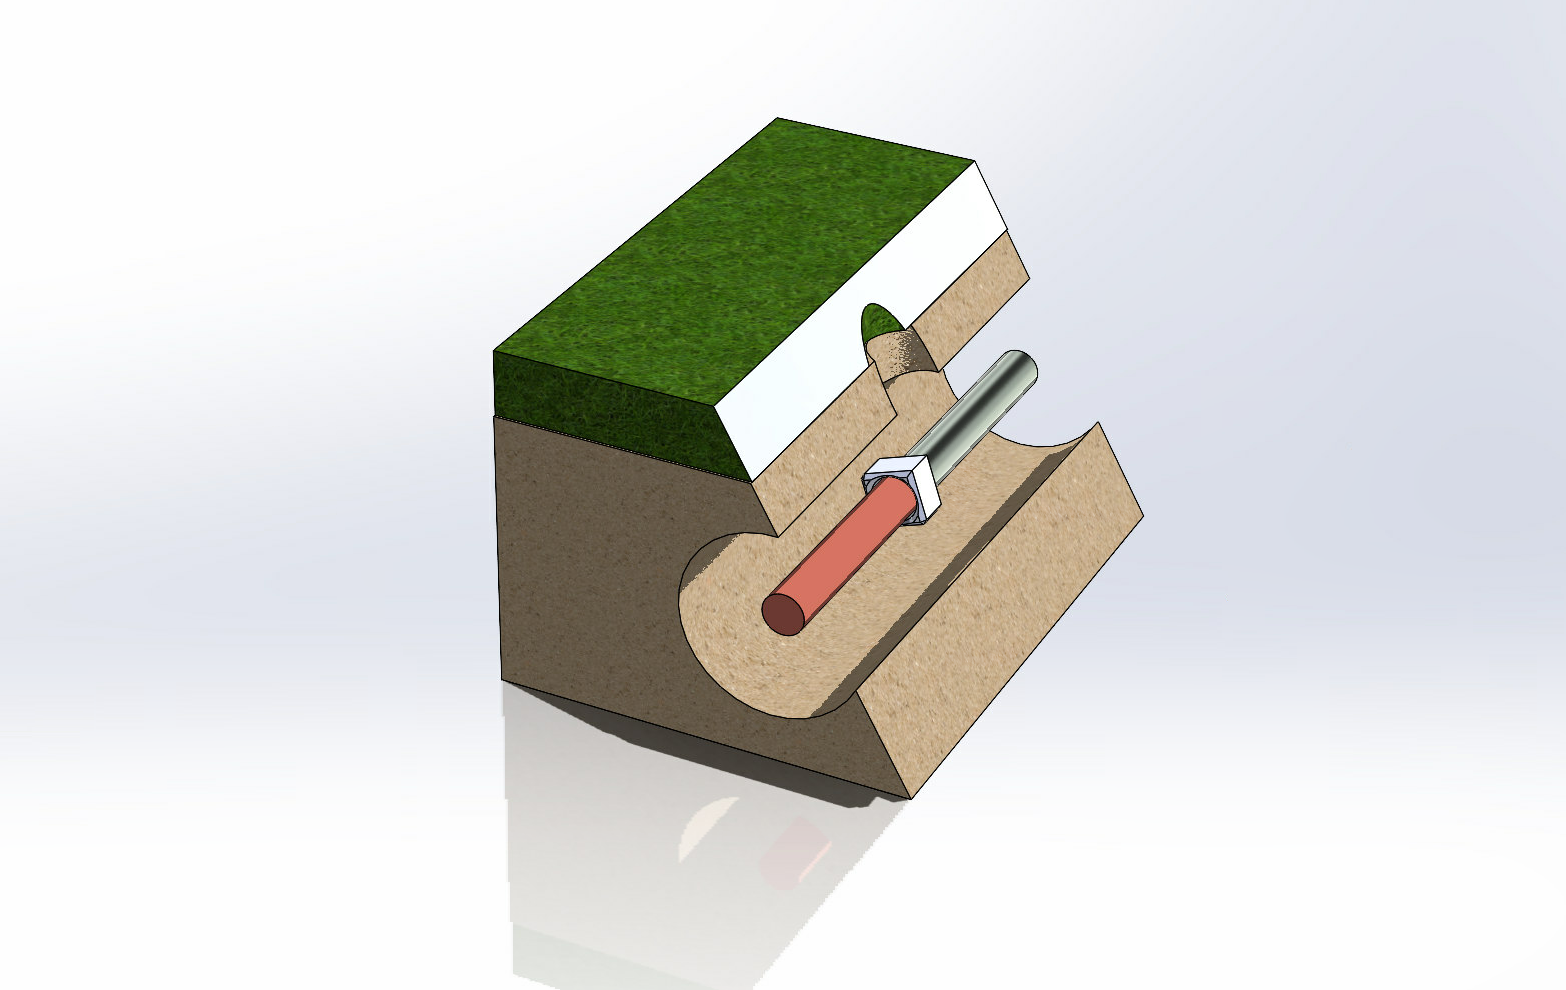
\includegraphics[width=\textwidth]{./Section_2.png}
        \caption{Section of the buried Copper and Lead Pipe}
        \label{fig:sub1}
    \end{subfigure}
    \hfill
    \begin{subfigure}[b]{0.4\textwidth}
        \centering

        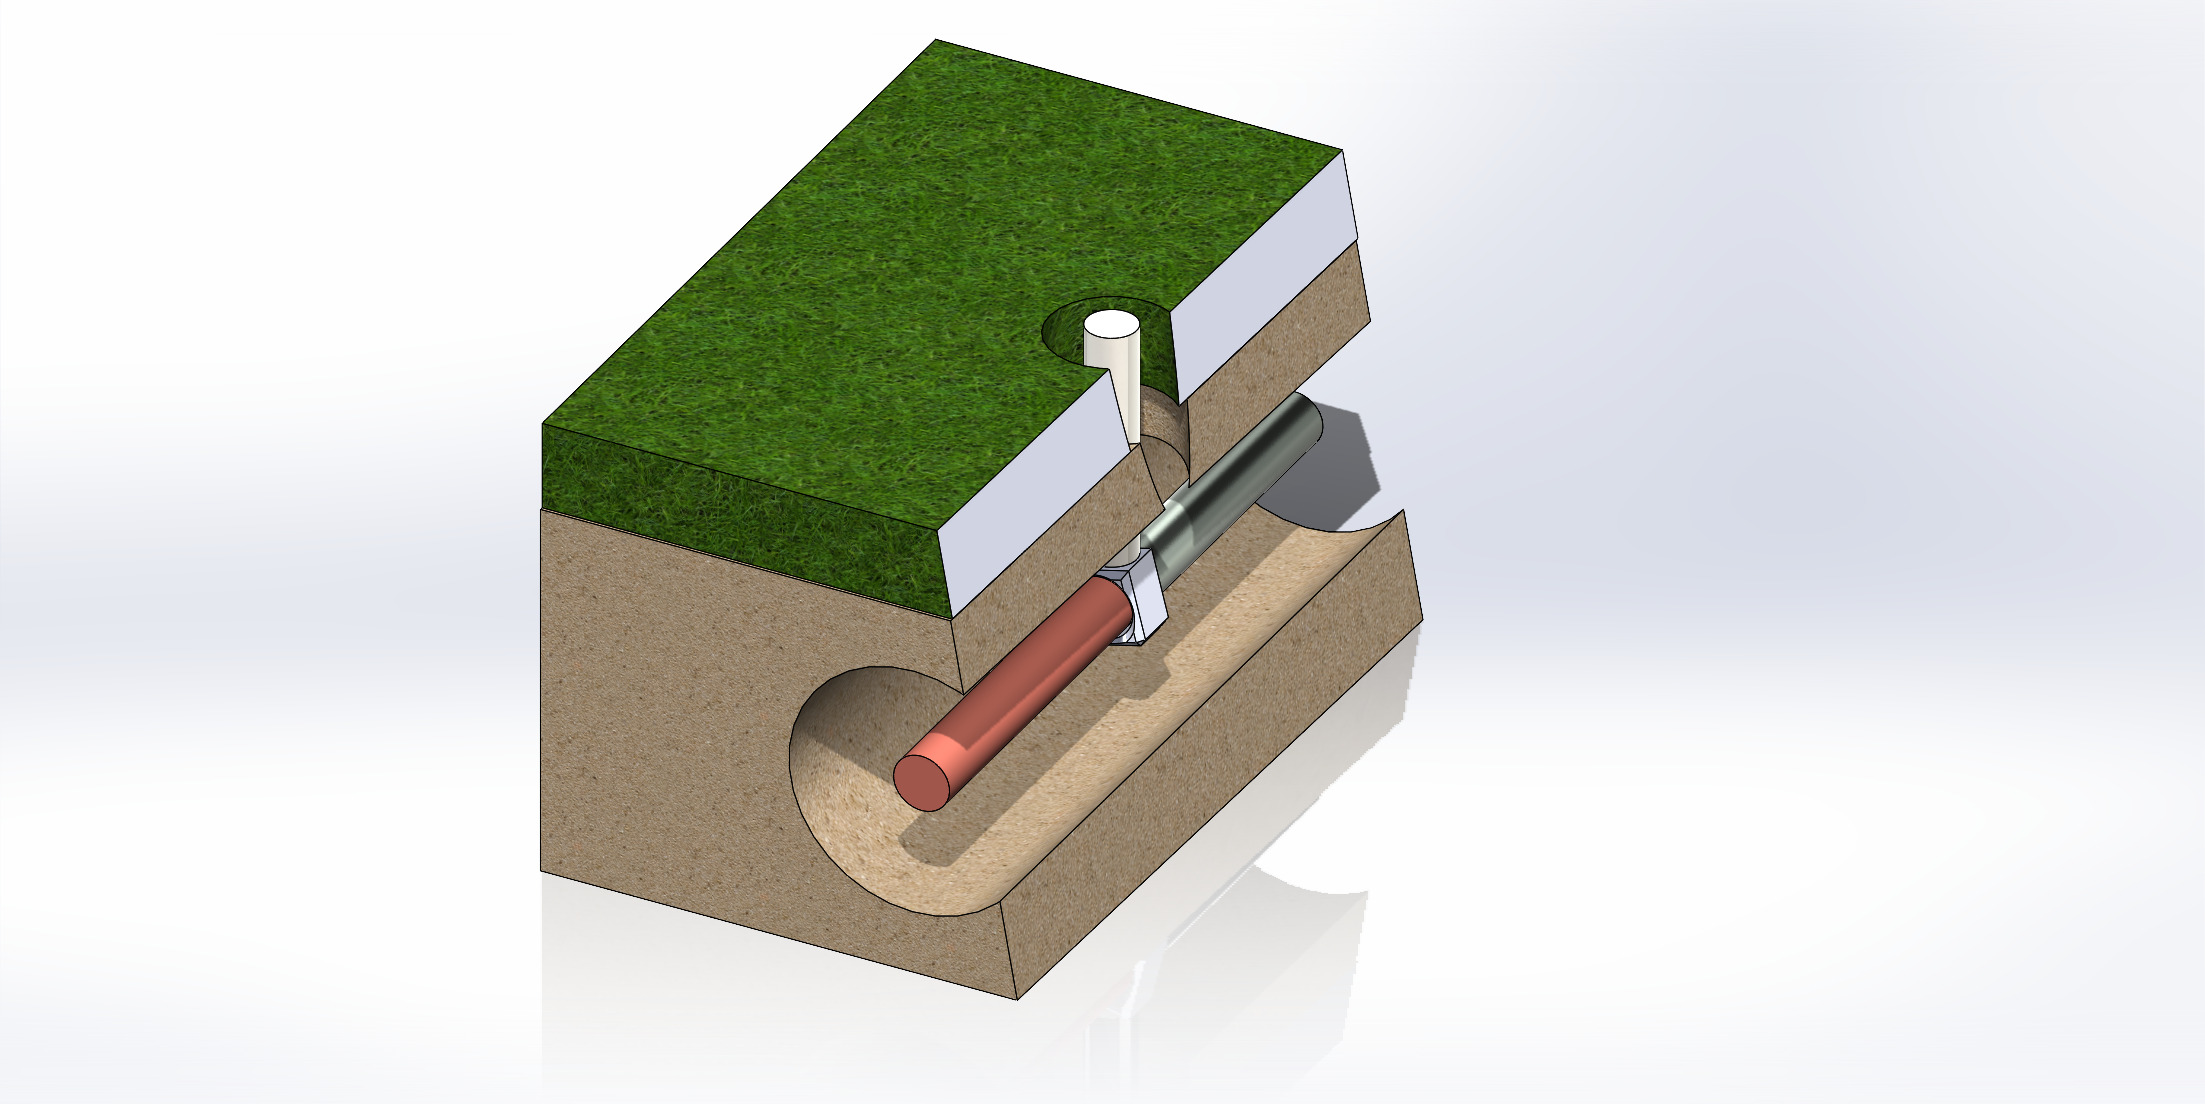
\includegraphics[width=\textwidth]{./Complete.jpg}
        \caption{Top View}
        \label{fig:sub2}
    \end{subfigure}
    \caption{Section of the buried Copper and Lead Pipe with steel rod}
    \label{fig:main}
\end{figure}



\subsection{Dataset Generation}
Approximately 5000 datasets were generated to train the machine learning model. The large dataset is critical for improving the accuracy and reliability of the CNN used for detection.

\begin{figure}[t]
    \centering
    \begin{subfigure}[b]{0.4\textwidth}
        \centering
        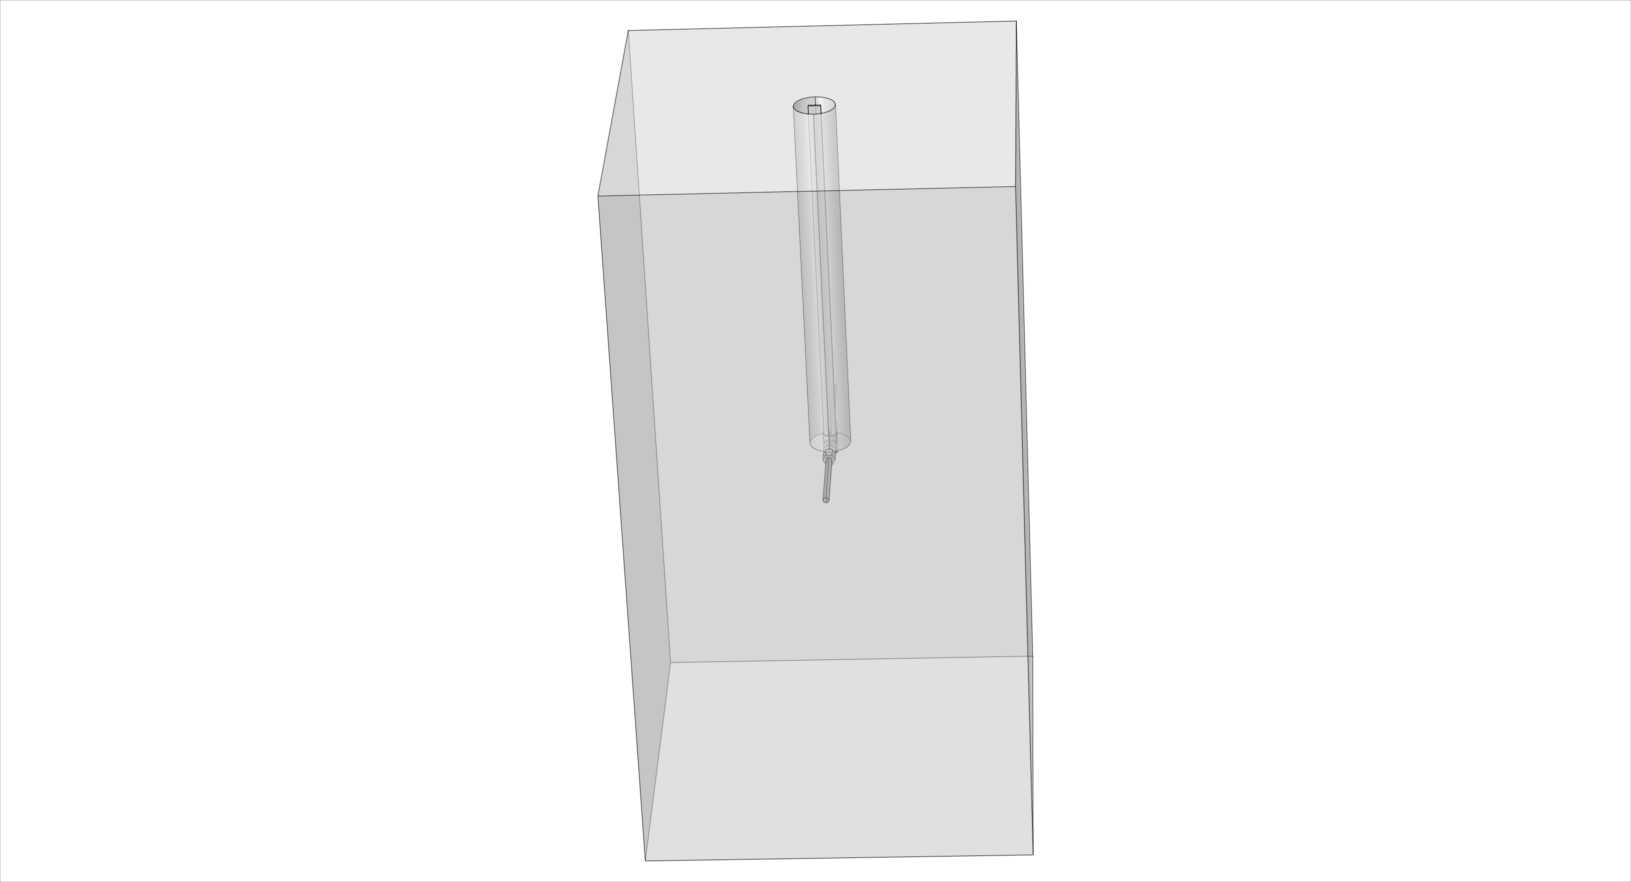
\includegraphics[width=\textwidth]{./Model_Image.png}
        \caption{Side View}
        \label{fig:sub1}
    \end{subfigure}
    \hfill
    \begin{subfigure}[b]{0.4\textwidth}
        \centering
        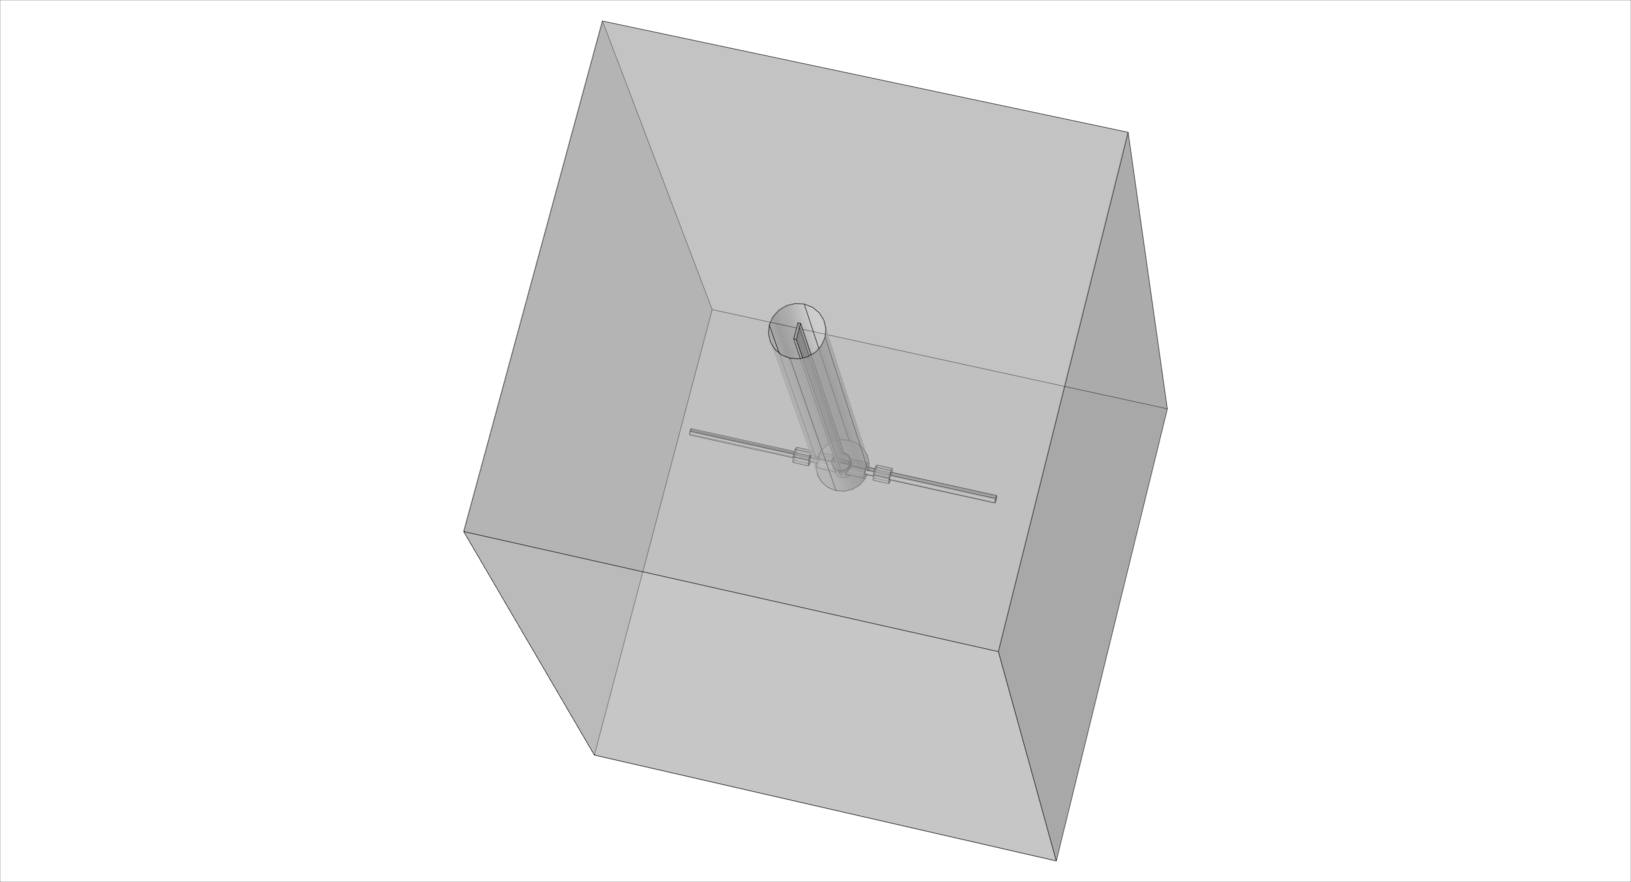
\includegraphics[width=\textwidth]{./Model_Image_12.png}
        \caption{Top View}
        \label{fig:sub2}
    \end{subfigure}
    \caption{Side and Top View of the Solid}
    \label{fig:main}
\end{figure}


\begin{equation}
  \rho \left( \frac{\partial^2 u}{\partial t^2} \right) = \nabla \cdot \mathbf{S} + \mathbf{F}_v
\end{equation}


\subsubsection{Data Categorization}
The generated data was separated into two categories: lead and copper. This categorization enabled the CNN to learn the distinct characteristics of each metal.

\subsubsection{Model Training}
The categorized data was used to train the CNN, aiming to develop a robust detection system capable of identifying the presence of lead and copper in buried pipes.

 

% Uncomment for bibliography on each chapter.
% \bibliographystyle{plainnat}				
% \markright{\textit{Bibliography}}
% \renewcommand{\chaptername}{}
% \bibliography{my_references}

% \vfill


%%% Local Variables:
%%% mode: latex
%%% TeX-master: "DMSE-Thesis"
%%% End:

\chapter{Results}
\noindent
\section{Computational Results}

The integration of COMSOL simulations with machine learning resulted in a comprehensive dataset representing various real-world scenarios. The CNN was trained with this data, showing promising accuracy in distinguishing between lead and copper based on the recorded acceleration readings.


\begin{table}[h]
\centering
\begin{tabular}{|r|r|}
  Description & Point graph\\
  
  X & Height\\
  0 & 5.817362260551916E-20\\
  1 & 5.817362260551916E-20\\
  2 & 6.046114033737459E-20\\
  3 & 5.076492751732623E-20\\
  4 & 2.0101101950650483E-20\\
  5 & 6.082783728329581E-20\\
  6 & 6.082783728329581E-20\\
  7 & 6.082783728329579E-20\\
  8 & 1.3190892577783899E-20\\
  9 & 4.7556868646350063E-20\\
  10 & 4.755686864635008E-20\\
  11 & 4.7556868646350033E-20\\
\end{tabular}

\caption{Result of Lead and Copper after Sinusoidal load has been applied.}
\label{tab:result}
\end{table}



\begin{figure}[t]
  \centering
  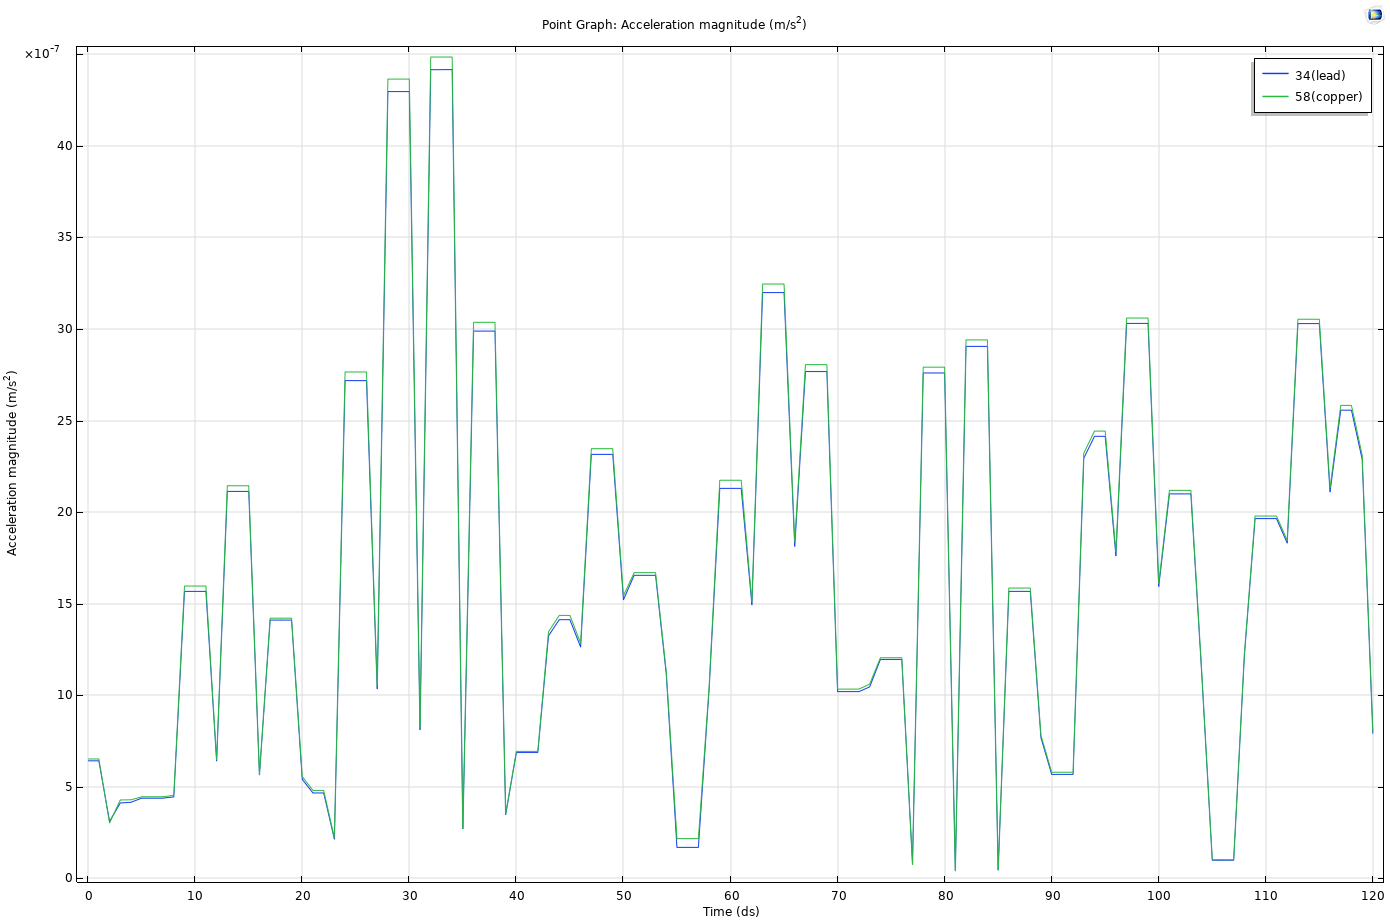
\includegraphics[width=0.4\hsize]{./Graph.png}
  \caption{The graph that distinguishes between lead and copper.}
  \label{fig:logo}
\end{figure}

% Uncomment for bibliography on each chapter.
% \bibliographystyle{plainnat}				
% \markright{\textit{Bibliography}}
% \renewcommand{\chaptername}{}
% \bibliography{my_references}

% \vfill


%%% Local Variables:
%%% mode: latex
%%% TeX-master: "DMSE-Thesis"
%%% End:

\chapter{Discussion}

\noindent

The combined use of COMSOL and machine learning demonstrated significant potential in improving the efficiency and accuracy of metal detection in water systems. The enhanced model, which includes a soil block and steel rod, effectively simulates real-world conditions. The generated dataset and subsequent training of the CNN highlight the feasibility of this approach. However, the process was slowed by the computational resources required, indicating a need for optimization in future work.

% Uncomment for bibliography on each chapter.
% \bibliographystyle{plainnat}				
% \markright{\textit{Bibliography}}
% \renewcommand{\chaptername}{}
% \bibliography{my_references}


% \vfill


%%% Local Variables:
%%% mode: latex
%%% TeX-master: "DMSE-Thesis"
%%% End:

\chapter{Conclusions}
\noindent
This study presents a novel method for detecting lead and copper in buried pipes by integrating COMSOL simulations with machine learning techniques. The enhanced model and extensive dataset generation contribute to a more accurate and efficient detection system. Future work will focus on optimizing the computational aspects and further validating the model with real-world data.

% Uncomment for bibliography on each chapter.
% \bibliographystyle{plainnat}				
% \markright{\textit{Bibliography}}
% \renewcommand{\chaptername}{}
% \bibliography{my_references}

% \vfill

%%% Local Variables:
%%% mode: latex
%%% TeX-master: "DMSE-Thesis"
%%% End:

\chapter{Future Research}
\label{ch:Fr}

Extensive field testing and validation in various environments would be crucial to ensure the model's robustness and accuracy in real-world conditions. Collaborations with environmental agencies or institutions for large-scale validation studies could provide valuable insights and further enhance the model's reliability.


% Uncomment for bibliography on each chapter.
% \bibliographystyle{plainnat}				
% \markright{\textit{Bibliography}}
% \renewcommand{\chaptername}{Future Works}
% \bibliography{my_references}

% \vfill


%%% Local Variables:
%%% mode: latex
%%% TeX-master: "DMSE-Thesis"
%%% End:



\bibliography{reference.bib}





% \vfill


%%% Local Variables:
%%% mode: latex
%%% TeX-master: "DMSE-Thesis"
%%% End:

\appendix
\include{app_pprofile} % HHP profile
\include{app_specimens} % master list
\include{app_thesis_prep} % programs used to generate this document
\include{app_figs} % list of microscope figures used in text


% 

% You can choose between:

% (a) One bibliography at the end of the document. This is appropriate
% for numbered citations (default).
\bibliographystyle{plainnat}	

% You can choose the title of the bibliography here:
% \renewcommand{\bibname}{My Own Title for References}


% (b) One bibliography at the end of the document plus a bibliography
% for each chapter. This only makes sense for "naming" bibliography
% styles, not for "numbering" styles: A style with numbering will give
% separate and unrelated numbers in each bibliography.

% This chooses an unnumbered bibliography style. 
% \bibliographystyle{unsrt} 

% You can choose the title of the global bibliography here:
% \renewcommand{\bibname}{Complete References}

% Include/uncomment the following lines at the end of each chapter .tex file:
% \bibliographystyle{plainnat}				
% \markright{\textit{Bibliography}}
% \renewcommand{\chaptername}{}
% \bibliography{my_references}

% To generate all bibliographies, proceed as follows:
% (1) Activate package chapterbib with option rootbib.
% \usepackage[rootbib]{chapterbib}
% (2) Run LaTeX.
% (3) Run BibTeX on the root file.
% (4) Deactivate option rootbib (i.e. load package without that option).
% \usepackage{chapterbib}
% (5) Run LaTeX.
% (6) Run BibTeX on each included file.
% (7) Run LaTeX twice.


\end{document}
\end


% Local Variables: 
% mode: tex-pdf
% TeX-master: t
% End: 


				


